\documentclass[12pt]{article}  

%%%%%%%% LIBRERIAS %%%%%%%%%%%%
\title{Plantilla para Tesina}
\usepackage[spanish]{babel} %Indica que escribiermos en español
\usepackage[utf8]{inputenc} %Indica qué codificación se está usando ISO-8859-1(latin1)  o utf8  
%Para agregar citas en apa
%Para citar se usa el comando \cite{}
%Las referencias se modifican en el archivo biblio.bib
\usepackage{apacite}
%----------------------------------------------

\usepackage{amsmath} % Comandos extras para matemáticas (cajas para ecuaciones,
% etc)
\usepackage{amssymb} % Simbolos matematicos (por lo tanto)
\usepackage{graphicx} % Incluir imágenes en LaTeX
\usepackage{color} % Para colorear texto
\usepackage{subfigure} % subfiguras
\usepackage{float} %Podemos usar el especificador [H] en las figuras para que se
% queden donde queramos
\usepackage{capt-of} % Permite usar etiquetas fuera de elementos flotantes
% (etiquetas de figuras)
\usepackage{sidecap} % Para poner el texto de las imágenes al lado
	\sidecaptionvpos{figure}{c} % Para que el texto se alinie al centro vertical
%\usepackage{caption} % Para poder quitar numeracion de figuras
\usepackage[font=small, labelfont=bf]{caption}
\usepackage{commath} % funcionalidades extras para diferenciales, integrales,
% etc (\od, \dif, etc)
\usepackage{cancel} % para cancelar expresiones (\cancelto{0}{x})
 
\usepackage{anysize} 					% Para personalizar el ancho de  los márgenes
\marginsize{1.91cm}{1.91cm}{2.54cm}{2.54cm} % Izquierda, derecha, arriba, abajo
\setlength{\parskip}{5mm} %indica el espaciado entre paginas
\usepackage{amsmath, amssymb, latexsym}
\usepackage{wrapfig,booktabs}


% Para que las referencias sean hipervínculos a las figuras o ecuaciones y
% aparezcan en color
%\usepackage[colorlinks=true,plainpages=true,citecolor=blue,linkcolor=blue]{hyperref}
%\usepackage{hyperref} 
% Para agregar encabezado y pie de página
\usepackage{fancyhdr} 
\pagestyle{fancy}
\fancyhf{}
\fancyhead[L]{\footnotesize Universidad de Guadalajara} %encabezado izquierda
\fancyhead[R]{\footnotesize CUCEI}   % dereecha
\fancyfoot[R]{\footnotesize Trabajo Final}  % Pie derecha
\fancyfoot[C]{\thepage}  % centro
\fancyfoot[L]{\footnotesize Monzón de Norteamérica}  %izquierda
\renewcommand{\footrulewidth}{0.4pt}


\title{Plantilla para Reportes}
% Basada en otra UPT  Overleaf

%%%%%%%% TERMINA LIBRERIAS%%%%%%%%%%%%

\begin{document}

%%%%%%%%%%%%%%%%%%%%%%%%%%% PORTADA %%%%%%%%%%%%%%%%%%%%%%%%
																					%%%
\begin{center}																		%%%
\newcommand{\HRule}{\rule{\linewidth}{0.5mm}}									%%%\left
 																					%%%
\begin{minipage}{0.48\textwidth} \begin{flushleft}

\includegraphics[scale = 0.05]{Imagenes/Escudo_UdeG.png}
\end{flushleft}\end{minipage}
\begin{minipage}{0.48\textwidth} \begin{flushright}

\includegraphics[scale = 0.09]{Imagenes/Escudo_CUCEI.png}
\end{flushright}\end{minipage}

													 								%%%
\vspace*{0.7cm}								%%%
																					%%%	
\textsc{\huge Maestría en Ciencias  \\ \vspace{5px} en Hidrometeorología}\\[1.5cm]	

\textsc{\LARGE Meteorología Tropical  }\\[1.5cm]													%%%

\begin{minipage}{0.9\textwidth} 
\begin{center}																					%%%
\textsc{\LARGE Trabajo Final }
\end{center}
\end{minipage}\\[0.5cm]
%%%
    																				%%%
 			\vspace*{1cm}																		%%%
																					%%%
\HRule \\[0.4cm]																	%%%
{ \huge \bfseries El Monzón de Norteamérica}\\[0.4cm]	%%%
 																					%%%
\HRule \\[1.5cm]																	%%%															%%%
\begin{center}	\large											%%%										%%%

% Aqui a continuación pongan los nombres de los integrantes
\emph{Alumno:}\\	
Joyce Ibeth Casanova Chacón\\
                        
\end{center}		
                              %%%
					\vspace{0.5cm} 											%%%
\begin{center}	\large	
\vspace{-0.6cm}											%%%															%%%
\emph{Profesor:} \\																	%%%
Dr. Faustino Omar García Concepción\\																									%%%
\end{center}	
\vspace*{1cm}


\vspace{1cm} 																				
\begin{center}	
Guadalajara, Jal. \\
{\large \today}																	%%%
 			\end{center}												  						
\end{center}	
\thispagestyle{empty} % Impide que se incluya número de página en la portada
\clearpage\setcounter{page}{1} % Comienza a incluir números de página a partir de aquí
\pagenumbering{roman} % En números romanos
%%%%%%%%%%%%%%%%%%%% TERMINA PORTADA %%%%%%%%%%%%%%%%%%%%%%%%%%%%%
\newpage
\tableofcontents

\newpage
\listoffigures

\newpage
\clearpage\setcounter{page}{1} % Comienza a incluir números de página a partir de aquí
\pagenumbering{arabic}
\section{Introducción}

En este trabajo se aborda el tema del Monzón de Norteamérica (NAM por sus siglas en inglés), el cual afecta la costa este de los Estados Unidos de América (EE.UU.) y los estados del noroeste de México.

El origen de la palabra monzón proviene del árabe clásico mawsi, que significa temporada. Los antiguos comerciantes que navegaban por el Océano Índico y el Mar Arábigo lo usaban para describir un sistema de vientos alternos que soplan persistentemente desde el noreste durante el invierno y desde la dirección opuesta, el suroeste, durante el verano.

Ahora se sabe que las inversiones estacionales de la dirección del viento ocurren debido a las diferencias de temperatura entre la tierra y el mar en todos los trópicos. Hay muchas características en común en estas circulaciones de monzones de verano, pero las más reconocibles son los cambios estacionales en los patrones de precipitación: lluvias con un flujo hacia tierra en verano y tiempo seco con flujo hacia el mar en invierno \cite{COMET}.

Se define el área del monzón como las regiones que abarcan las circulaciones superficiales de enero y julio en las que \cite{ramage-1971}:

\begin{itemize}
\item La dirección del viento dominante cambia al menos 120°. 
\item Frecuencia media del viento dominante superior al 40\%.
\item Velocidad media del viento en al menos uno de los meses supera los 3 ms$^{-1}$.
\item Patrones de presión que satisfacen un criterio de vientos constantes (menos de una alternancia ciclón-anticiclón ocurre cada dos años en cualquier mes en un rectángulo de 5° de latitud y longitud).
\end{itemize}

Si bien las características típicas descritas en la definición de Ramage (1971) las presenta el monzón de la India, después  se han reconocido otras regiones monzónicas, y en tiempos más actuales se ha incluido algunas regiones del continente Americano. 

La importancia de estudiar los monzones alrededor del mundo es fundamental, debido a que muchas sociedades dependen de este régimen de precipitación. El monzón de Norteamérica afecta una de las zonas de más rápido crecimiento en los EE.UU. y en México, las tormentas generadas por el sistema monzónico pueden traer lluvias beneficiosas y vivificantes. Sin embargo, dichas lluvias también pueden ser mortales, ya que desencadenan repentinas inundaciones, decargas eléctricas, granizo que daña las cosechas, así como intensos vientos.


\section{Capítulo 1. El Monzón De Norteamérica}

\subsection{Regiones Monzónicas}

A partir de la definición dada por Ramage, las regiones monzónicas en el mundo que cumplen los cuatro criterios se muestran a continuación en la Figura  \ref{fig:Regiones Monzónicas}:

\begin{figure}[H]
	\begin{center}
 		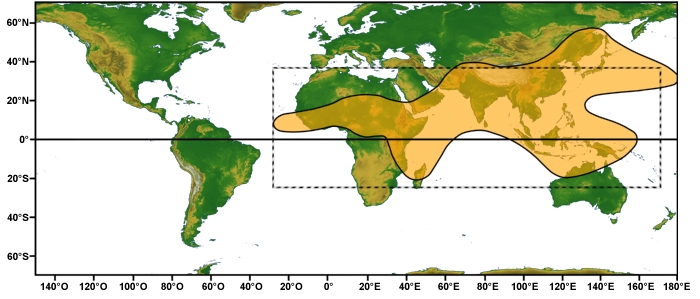
\includegraphics[width = 1\textwidth]{Imagenes/monsoonregions.jpg}
 		\captionof{figure}{\label{fig:Regiones Monzónicas}Regiones Monzónicas con base en la definición de Ramage (1971). El área sombreada es monzónica de acuerdo con el criterio de viento en superficie, el rectángulo encierra las regiones monzónicas que satisfacen los 4 cirterios de la definición clásica.}Fuente: \cite{COMET}.	
	\end{center} 
\end{figure}

En la actualidad, entre los sistemas monzónicos mundiales se incluyen algunas regiones del continente americano donde las características de precipitación y vientos son similares a los de los monzones clásicos de Australia, India y el sudeste asiático. Sin embargo, las inversiones estacionales del viento son menos pronunciadas sobre las Américas que en otras partes del mundo \cite{CPC} . Como se muestra en la Figura \ref{fig:Sistemas monzónicos}, dichas regiones no tienen un equivalente de invierno, de modo que no se ajustan plenamente a los criterios clásicos que definen los monzones.

\begin{figure}[H]
	\begin{center}
 		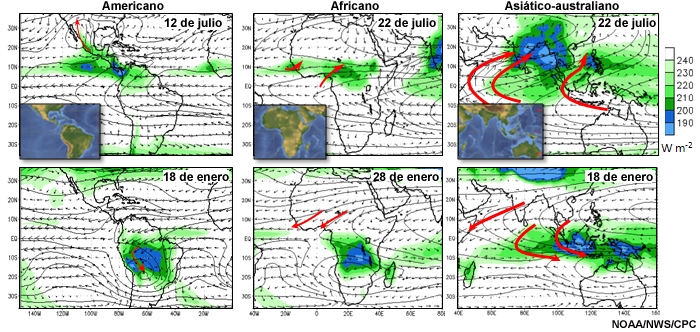
\includegraphics[width = 0.8\textwidth]{Imagenes/global_monsoons.jpg}
 		\captionof{figure}{\label{fig:Sistemas monzónicos}Sistemas Monzónicos. Radiación de OL saliente, líneas de corriente en 200 hPa, climatología de vientos en 850 hPa (1979-1995).}
 		Fuente: \cite{COMET} 
	\end{center} 
\end{figure}

\subsection{El Monzón de Norteamérica}

El monzón de Norteamérica, también conocido como monzón del suroeste de los Estados Unidos o monzón mexicano, es un cambio estacional en la circulación atmosférica, que se manifiesta como un aumento pronunciado de las precipitaciones desde un junio extremadamente seco hasta un julio lluvioso en amplias zonas del suroeste de Estados Unidos y el noroeste de México. Estas lluvias de verano suelen durar hasta mediados de septiembre, cuando se restablece un régimen más seco sobre la región \cite{adams1997north}.

Este fenómeno influye en áreas grandes del suroeste de EE.UU. (Arizona y Nuevo México, principalmente), y tiene su centro sobre el noroeste México; en la Figura \ref{fig:Regiones de influencia del NAM} se muestran los rasgos fisiográficos y estados de ambos países que se relacionan con el NAM.

El calentamiento sobre las montañas de México y el oeste de EE.UU. juega un papel importante en el desarrollo y evolución del monzón \cite{CPC}. El monzón comienza a desarrollarse en México en junio y avanza hacia el suroeste de los EE. UU. en julio. Desde principios hasta mediados de septiembre, los patrones de viento generalmente han vuelto al patrón del oeste, poniendo fin al monzón \cite{Climategov}.

\begin{figure}[H]
	\begin{center}
 		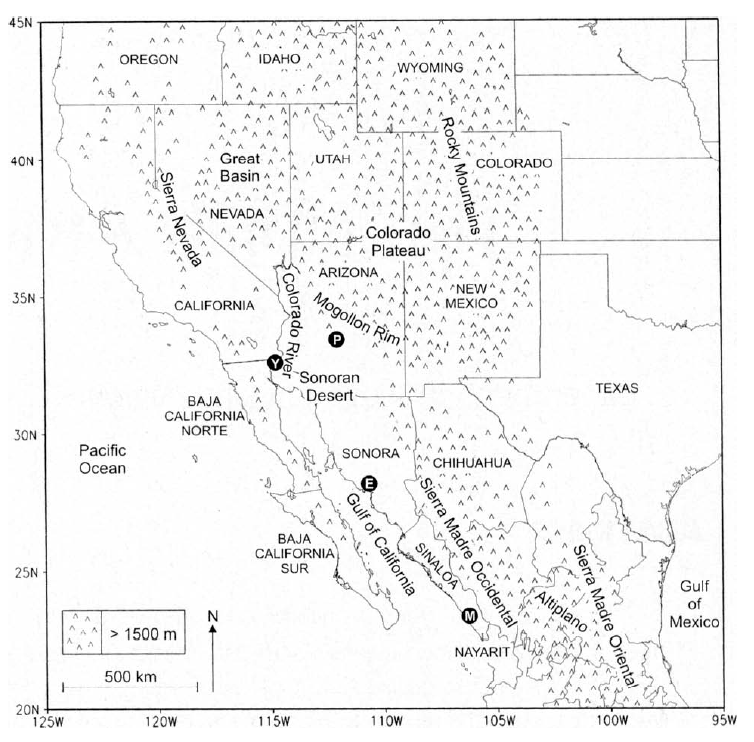
\includegraphics[width = 0.45\textwidth]{Imagenes/Regiones de influencia NAM.png}
 		\captionof{figure}{\label{fig:Regiones de influencia del NAM}Principales fisiográficos del suroeste de América del Norte que se relacionan con el NAM. Menciones en la imagen: Empalme (E), Mazatlán (M), Phoenix (P), y Yuma (Y).} 
 		Fuente: \cite{adams1997north}.
	\end{center} 
\end{figure}

A medida que el calor del verano se acumula en América del Norte, se forma una región de alta presión en el suroeste de los EE. UU. y el viento se vuelve más del sur, trayendo humedad del Océano Pacífico, el Golfo de California y del Golfo de México \cite{COMET2}, como se aprecia en los esquemas de la Figura \ref{fig:Esquemas NAM}. Esta circulación trae tormentas eléctricas y lluvias a la región del NAM, proporcionando gran parte de su precipitación total anual.

\begin{figure}[H]
	\begin{center}
 		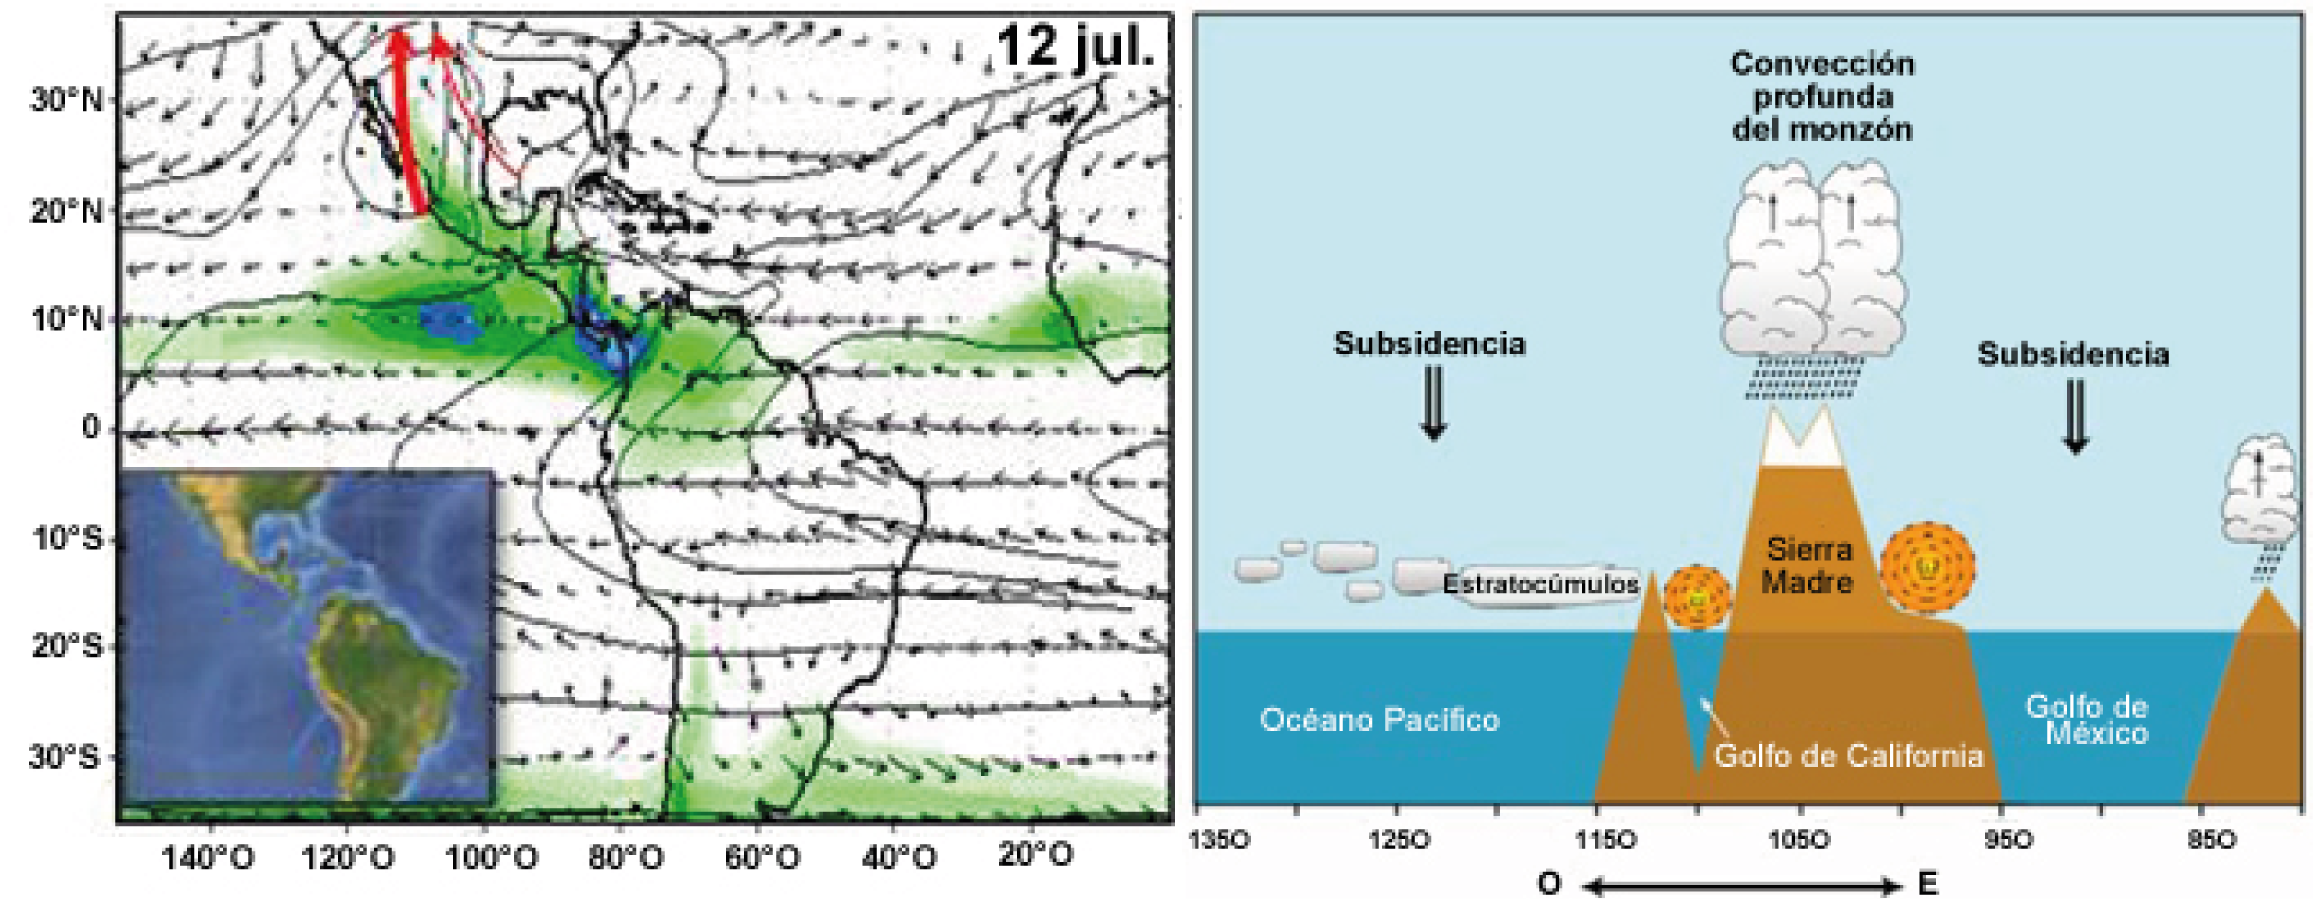
\includegraphics[width = 0.8\textwidth]{Imagenes/Esquemas NAM.png}
 		\captionof{figure}{\label{fig:Esquemas NAM}Izquierda: radiación de onda larga saliente, líneas de corriente en 200 hPa, vector viento en 850 hPa cerca del pico del NAM. Derecha: representación esquemática correspondiente al verano del NAM, de este a oeste a 30 grados de latitud norte. }
 		Fuente: \cite{COMET}.
	\end{center} 
\end{figure}

Con respecto al debate sobre las regiones de origen de la humedad y la advección del vapor de agua hacia el suroeste de América del Norte, existe un acuerdo general de que la mayor parte de la humedad del monzón se advecta a niveles bajos desde el Océano Pacífico tropical oriental y el Golfo de California, mientras que el Golfo de México puede contribuir con algo de humedad en los niveles superiores, aunque se produce una mezcla sobre la Sierra Madre Occidental \cite{Climategov}.

\subsection{Impactos del Monzón de Norteamérica en Noroeste de México y el Sureste de los EE.UU.}

Las precipitaciones asociadas al monzón son muy importantes para la región. El noroeste de México recibe de él más del 75\% de su precipitación media anual, mientras que Arizona y Nuevo México más del 50\%, durante los meses de julio a septiembre \cite{Climategov}, (ver Figura \ref{fig:Precipitación NAM}); esto pese a que la mayor parte de la precipitación generada por el monzón cae sobre el océano. La estación lluviosa del NAM dura aproximadamente 100 días \cite{COMET2}.

\begin{figure}[H]
	\begin{center}
 		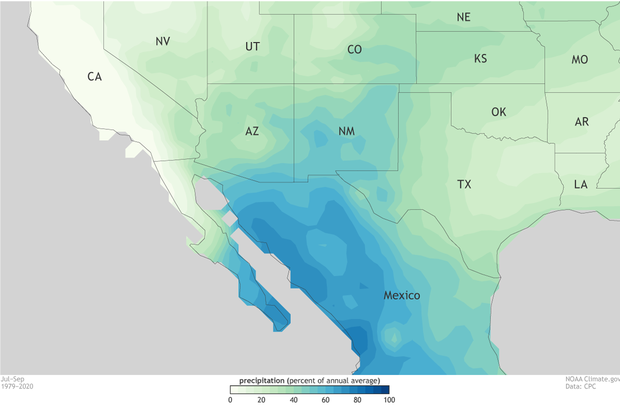
\includegraphics[width = 0.75\textwidth]{Imagenes/NAM_pct.png}
 		\captionof{figure}{\label{fig:Precipitación NAM}Porcentaje de precipitación anual total que ocurre durante el NAM (julio a septiembre), utilizando datos de pluviómetros unificados del CPC para el periodo 1979-2020.}
 		Fuente: \cite{Climategov}.
	\end{center} 
\end{figure}

En el NAM las precipitaciones suelen tener un fuerte ciclo diurno, es decir, un patrón diario de mañanas mayormente secas, tormentas que se desarrollan a lo largo del día y la mayor parte de las lluvias se producen por la tarde y la noche. Algunas de estas tormentas pueden ser fuertes, con fuertes lluvias y frecuentes relámpagos. La actividad de las lluvias monzónicas tiende a agruparse en ráfagas, con períodos de días lluviosos intercalados con períodos más secos, en lugar de lluvia todos los días. Además, las ocasionales tormentas tropicales del Pacífico oriental puede aumentar la humedad y las lluvias del monzón.

Los impactos del monzón van más allá de las cantidades de lluvia. También existe una relación importante entre la precipitación y la temperatura: por lo general, más lluvia genera condiciones más frías y menos lluvia genera condiciones más cálidas y secas, relacionando el NAM con los incendios forestales en el norte y noroeste de México, debido a que las lluvias monzónicas son importantes para acabar con los incendios forestales \cite{Climategov}.

\subsection{Variabilidad y factores que afectan el NAM}

Los aumentos repentinos de humedad en los niveles bajos procedentes del Golfo de California (GC) son una parte importante de la variabilidad intraestacional del NAM (ver Figura \ref{fig:Factores NAM}), y están asociados a la configuración de las vaguadas de latitudes medias en los niveles superiores, así como de las ondas tropicales (escala sinóptica), además de la presencia de chorros de niveles bajos, de una baja térmica y de la dinámica asociada (incluidos los importantes efectos de la topografía local) en la mesoescala \cite{adams1997north}.

\begin{figure}[H]
	\begin{center}
 		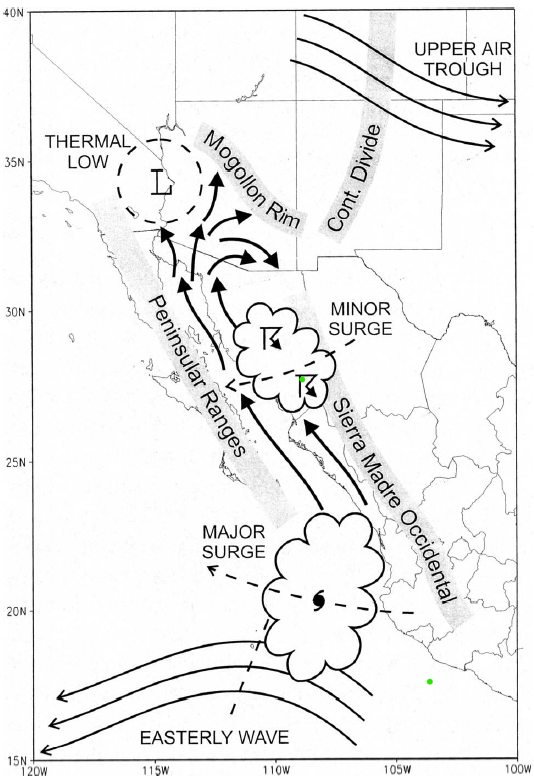
\includegraphics[width = 0.3\textwidth]{Imagenes/Humedad GC.png}
 		\captionof{figure}{\label{fig:Factores NAM}Conceptualización del fenómeno de aporte de humedad del Golfo de California.}
 		Fuente: \cite{adams1997north}.
	\end{center} 
\end{figure}

Algunos de los factores que influyen en la cantidad de humedad disponible para el monzón, son: la posición de la zona de alta presión, los patrones de viento y las características meteorológicas transitorias.

La variabilidad interanual del sistema monzónico de América del Norte es alta, pero no está fuertemente vinculada a El Niño Oscilación del Sur (ENSO por sus siglas en inglés), ni a otras fuentes comunes de variabilidad de la circulación interanual. Sin embargo, el ENSO influye en ciclones tropicales del Pacífico, que pueden aportar humedad al NAM \cite{Climategov}.

\subsection{Forzamiento mecánico del NAM por la orografía}

Al igual que en otros monzones tropicales, se cree comúnmente que este máximo de lluvia es forzado térmicamente por la emisión de calor desde la tierra y el terreno elevado hacia la atmósfera superior, pero se carece de una comprensión clara del mecanismo fundamental que gobierna este monzón. Debido a que, el monzón de Norteamérica se genera cuando las montañas de la Sierra Madre de México desvían la corriente en chorro extratropical hacia el ecuador, forzando mecánicamente el flujo cuesta arriba hacia el este que eleva el aire cálido y húmedo para producir lluvia convectiva \cite{boos2021}.

\subsection{Modelación del NAM}

Se requiere una comprensión física del NAM para guiar las mejoras en el modelado a escala regional y global de este monzón y sus impactos remotos en la circulación de verano y los patrones de precipitación en América del Norte. Aunque los modelos climáticos regionales han logrado reproducir algunas características de la NAM, su inicio, fuerza y extensión regional no están bien pronosticados. 

La modelación para el pronóstico del monzón de Norteamérica sigue siendo un reto para los distintos modelos numéricos disponibles, como se aprecia en la Figura \ref{fig:Modelación NAM}, donde la precipitación de vereno es generalmente menos pronosticada en la región del NAM \cite{DRI}.

\begin{figure}[H]
	\begin{center}
 		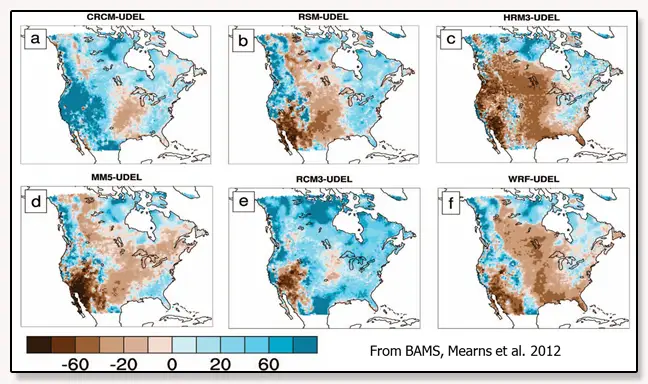
\includegraphics[width = 0.7\textwidth]{Imagenes/NAM1.png}
 		\captionof{figure}{\label{fig:Modelación NAM}El sesgo de precipitación de verano (diferencia \%; modelo-observación) para los modelos regionales.} Fuente: \cite{DRI}.
	\end{center} 
\end{figure}

\section{Conclusiones}


\begin{itemize}
\item El monzón de Norteamérica no se origina en la oscilación estacional de la Zona Intertropical de Convergencia (ZCIT por sus siglas en inglés), sobre las masas continentales como un monzón típico. Su origen representa un caso único, debido a que está fuertemente influenciado por la orografía de México, que desempeña un papel clave en la generación de una onda estacionaria en la circulación atmosférica extratropical y en el desvío de la corriente en chorro hacia la costa occidental mexicana.
\item  Los flujos de calor de la superficie terrestre precondicionan la atmósfera para la convección, particularmente en las tardes de verano, pero estos flujos de calor por sí solos son insuficientes para producir el máximo de lluvia observado. Por lo que se demuestra que el NAM debe entenderse como una lluvia orográfica mejorada por convección en una onda estacionaria forzada mecánicamente, no como un monzón tropical clásico forzado térmicamente.
\item  Las tendencias en las interacciones de las corrientes en chorro con la orografía son de importancia central para la respuesta del monzón de América del Norte al cambio climático global pasado y futuro.
\item  La amplia comprensión de la física del NAM es necesaria para predecir la respuesta del NAM ante el calentamiento global, así como para mejorar los modelos de pronóstico
\end{itemize}





% REFERENCIAS
%-------------------------------------------------------------------------------
\newpage

\bibliographystyle{apacite}
\bibliography{biblio.bib}


\end{document}
